\documentclass{standalone}
\usepackage{tikz}
\usetikzlibrary{arrows,decorations.markings,decorations.pathreplacing,calc,positioning}

% "Add arrows to a smooth tikz function"
% from http://tex.stackexchange.com/a/163695
\tikzset{
   set arrow inside/.code={\pgfqkeys{/tikz/arrow inside}{#1}},
   set arrow inside={end/.initial=>, opt/.initial=},
   /pgf/decoration/Mark/.style={
      mark/.expanded=at position #1 with
      {
         \noexpand\arrow[\pgfkeysvalueof{/tikz/arrow inside/opt}]{\pgfkeysvalueof{/tikz/arrow inside/end}}
      }
   },
   arrow inside/.style 2 args={
      set arrow inside={#1},
      postaction={
         decorate,decoration={
            markings,Mark/.list={#2}
         }
      }
   },
}

\ifdefined\argbeforeeval
   \def\drawoldaxes{}
   \def\drawotherold{}
   \def\drawevaledold{}
   \def\drawsharedold{}
\fi

\ifdefined\argselectcandidate
   \def\drawoldaxes{}
   \def\drawotherold{}
   \def\drawevaledold{}
   \def\drawsharedold{}
   \def\drawselectcandidate{}
\fi

\ifdefined\argnewcandidate
   \def\drawoldaxes{}
   \def\drawotherstale{}
   \def\drawsharedstale{}
   \def\drawevalednew{}
   \def\drawdeltap{}
   \def\drawdeltapline{}
\fi

\ifdefined\argnewshared
   \def\drawoldaxes{}
   \def\drawotherstale{}
   \def\drawevalednew{}
   \def\drawsharednew{}
   \def\drawdeltap{}
   \def\drawdeltapline{}
\fi

\ifdefined\argnewother
   \def\drawoldaxes{}
   \def\drawothernew{}
   \def\drawevalednew{}
   \def\drawsharednew{}
   \def\drawdeltap{}
   \def\drawdeltapline{}
\fi

\ifdefined\argnewaxes
   \def\drawnewaxes{}
   \def\drawothernew{}
   \def\drawevalednew{}
   \def\drawsharednew{}
   \def\drawdeltap{}
\fi

\begin{document}%
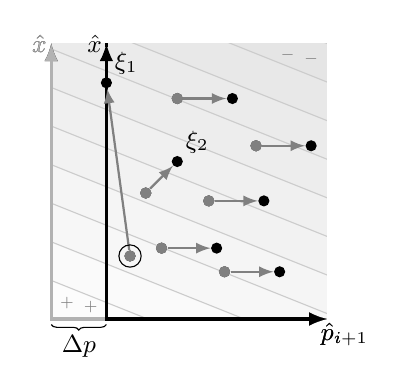
\begin{tikzpicture}[font=\small]

\clip (-0.3,-0.5) rectangle (4.1,3.7);

% contours
\begin{scope}
   \clip (0,0) rectangle (3.5,3.5);
   \foreach \s in {10,...,1}
   {
      \begin{scope}[shift={($(0.35*\s,0.35*\s)$)}]
      
         \draw[black!20,fill=black!\s]
         (-5.0,2.0) -- (5.0,-2.0)
          -- (-5.0,-2.0) -- cycle;
         
      \end{scope}
   }
\end{scope}

\node[text=black!50] at (0.2,0.20) {\tiny $+$};
\node[text=black!50] at (0.5,0.15) {\tiny $+$};
\node[text=black!50] at (3.0,3.35) {\tiny $-$};
\node[text=black!50] at (3.3,3.30) {\tiny $-$};

%\draw[black!5] (-0.1,-0.1) rectangle (3.6,3.6);

%\draw[black!50] (-0.1,0.7) -- (3.5,0.7); % optimal path
%\node at (1.75,0.9) {\scriptsize Optimal Path};

% simple point
%\node[circle,fill=black,inner sep=0.07cm] at (1.5,3) {};
%\node[circle,fill=black,inner sep=0.05cm] (a1) at (1.0,2.7) {};
%\node[above right=-0.1cm of a1] {$A_1$};

% anytime
%\draw[black,thick,->,
%   arrow inside={end=>,opt={black}}{0.25,0.5,0.75}]
%   (0.84,2.45)
%   .. controls (1.05,1.96) and (1.54,1.96) .. (1.96,1.75)
%   .. controls (2.38,1.54) and (2.67,0.84) .. (3.50,0.77);
%\node[circle,fill=black,inner sep=0.07cm] at (2.45,1.33) {};

% axes
\ifdefined\drawoldaxes
   \draw[black,very thick,latex-latex] (0,3.5) -- (0,0) -- (3.5,0);
   \node[anchor=west] at (3.3,-0.2) {$\hat p_i$};
   \node at (-0.15,3.5) {$\hat x$};
\fi

\ifdefined\drawnewaxes
   \draw[black!30,very thick,latex-latex] (0,3.5) -- (0,0) -- (3.5,0);
   % additional next-iteration axes
   \draw[black,very thick,latex-latex] (0.7,3.5) -- (0.7,0.0) -- (3.5,0);
   \node[anchor=west] at (3.3,-0.2) {$\hat p_{i+1}$};
   \node[text=black!30] at (-0.15,3.5) {$\hat x$};
   \node at (0.55,3.5) {$\hat x$};
\fi


% labels


\ifdefined\drawdeltap
   % label of p_sofar
   \draw [decorate,decoration={brace,amplitude=2pt,mirror},xshift=0pt,yshift=-2pt]
   (0.0,0.0) -- (0.7,0.0) node [inner sep=0pt,black,midway,yshift=-8pt] 
   {$\Delta p$};
\fi
\ifdefined\drawdeltapline
   \draw[black,very thick,densely dotted] (0.7,3.5) -- (0.7,0.0);
\fi

% some points

\ifdefined\drawevaledold
   \node[circle,fill=black,inner sep=0.05cm] (xi1old) at (1.0,0.8) {};
\fi
\ifdefined\drawevalednew
   \node[circle,fill=black!50,inner sep=0.05cm] (xi1old) at (1.0,0.8) {};
   \node[circle,fill=black,inner sep=0.05cm] (xi1) at (0.7,3.0) {};
   \draw[thick,-latex,black!50] (xi1old) -- (xi1);
   \node[above right=-0.1cm of xi1] {$\xi_1$};
\fi
\ifdefined\drawselectcandidate
   \node[circle,draw=black,inner sep=0.1cm] at (1.0,0.8) {};
\fi

\ifdefined\drawsharedold
   \node[circle,fill=black,inner sep=0.05cm] (xi2old) at (1.2,1.6) {};
\fi
\ifdefined\drawsharedstale
   \node[circle,fill=black!50,inner sep=0.05cm] (xi2old) at (1.2,1.6) {};
\fi
\ifdefined\drawsharednew
   \node[circle,fill=black!50,inner sep=0.05cm] (xi2old) at (1.2,1.6) {};
   \node[circle,fill=black,inner sep=0.05cm] (xi2) at (1.6,2.0) {};
   \draw[thick,-latex,black!50] (xi2old) -- (xi2);
   \node[above right=-0.1cm of xi2] {$\xi_2$};
\fi

\ifdefined\drawotherold
   \node[circle,fill=black,inner sep=0.05cm] (xi3old) at (2.2,0.6) {};
   \node[circle,fill=black,inner sep=0.05cm] (xi4old) at (2.0,1.5) {};
   \node[circle,fill=black,inner sep=0.05cm] (xi5old) at (1.6,2.8) {};
   \node[circle,fill=black,inner sep=0.05cm] (xi6old) at (2.6,2.2) {};
   \node[circle,fill=black,inner sep=0.05cm] (xi7old) at (1.4,0.9) {};
\fi

\ifdefined\drawotherstale
   \node[circle,fill=black!50,inner sep=0.05cm] (xi3old) at (2.2,0.6) {};
   \node[circle,fill=black!50,inner sep=0.05cm] (xi4old) at (2.0,1.5) {};
   \node[circle,fill=black!50,inner sep=0.05cm] (xi5old) at (1.6,2.8) {};
   \node[circle,fill=black!50,inner sep=0.05cm] (xi6old) at (2.6,2.2) {};
   \node[circle,fill=black!50,inner sep=0.05cm] (xi7old) at (1.4,0.9) {};
\fi

\ifdefined\drawothernew
   \node[circle,fill=black!50,inner sep=0.05cm] (xi3old) at (2.2,0.6) {};
   \node[circle,fill=black,inner sep=0.05cm] (xi3) at (2.9,0.6) {};
   \draw[thick,-latex,black!50] (xi3old) -- (xi3);

   \node[circle,fill=black!50,inner sep=0.05cm] (xi4old) at (2.0,1.5) {};
   \node[circle,fill=black,inner sep=0.05cm] (xi4) at (2.7,1.5) {};
   \draw[thick,-latex,black!50] (xi4old) -- (xi4);

   \node[circle,fill=black!50,inner sep=0.05cm] (xi5old) at (1.6,2.8) {};
   \node[circle,fill=black,inner sep=0.05cm] (xi5) at (2.3,2.8) {};
   \draw[thick,-latex,black!50] (xi5old) -- (xi5);

   \node[circle,fill=black!50,inner sep=0.05cm] (xi6old) at (2.6,2.2) {};
   \node[circle,fill=black,inner sep=0.05cm] (xi6) at (3.3,2.2) {};
   \draw[thick,-latex,black!50] (xi6old) -- (xi6);

   \node[circle,fill=black!50,inner sep=0.05cm] (xi7old) at (1.4,0.9) {};
   \node[circle,fill=black,inner sep=0.05cm] (xi7) at (2.1,0.9) {};
   \draw[thick,-latex,black!50] (xi7old) -- (xi7);
\fi



%\node at (-0.2,0.75) {$x^*$};

%\node[anchor=east,inner sep=0pt] at (3.5,0.2) {\scriptsize Planning Effort $\rightarrow$};
%\node[rotate=90,anchor=east,inner sep=0pt] at (0.2,3.5) {\scriptsize Execution Effort $\rightarrow$};

\end{tikzpicture}%
\end{document}
